


This section will summarise the results of the scientific papers the dissertation is based on. All papers utilised some version of the LT-FH++, which will be referred to as age-dependent liability threshold model when no family history is being used. Each paper has its own distinct use case of the model, which will be highlighted in the coming sections.

\section{Paper 1 - LT-FH++}
The first paper proposed the method LT-FH++, which is an extension of the previously proposed LT-FH method by Hujoel et al\cite{hujoel2020liability}. The notable difference between LT-FH and LT-FH++ is the ability to account for age of onset for cases or age for controls, sex, and birth year, as well as the same information in the included family members. The LT-FH method does not consider sex or age in parents, meaning they have the same thresholds. It also uses the same threshold for the index person and siblings and does not distinguish on age or sex differences. LT-FH++ is also able to account for siblings individually rather than considering the number of siblings and an \enquote{\textit{at least one affected sibling}} indicator. This way of coding siblings in LT-FH is likely due to the way sibling information is coded in the UKBB, which was the main application of the LT-FH paper. Considerable changes have also been made to the sampling strategy to allow for the increased flexibility in the family and the use of personalised thresholds to be scalable to millions of individuals.  The changes LT-FH++ proposed increased the number of unique configurations considerably, as each individual now has a unique set of family members and thresholds. The sampling strategy used for LT-FH would be computationally intractable for LT-FH++, since LT-FH only needed to estimate a liability for a handful of configurations.


\subsection{Simulation results}
We performed simulations to assess the power and false discovery rate of LT-FH++ against LT-FH and a case-control status to detect causal SNPs in a linear regression GWAS. The simulations are based on simulated genotypes, where we simulated a pair of parents and one offspring with no siblings. We used parameters similar to the ones used in the LT-FH paper to ensure compatibility between findings. The simulated genotypes had a heritability on the liability scale of $ h^2 = 0.5 $, a population prevalence of $ 5\% $. Unlike in the LT-FH paper, we used a higher prevalence in one of the simulated sexes, but the combined prevalence would still be $ 5\% $. The case ratio was $ 1{\,:\,}4 $ between sexes, and it was also present in the parents. We also considered a population prevalence of $ 10\% $, but those results are not shown here. The genotypes consisted of $ 100,000 $ individuals, each with $ 100,000 $ independent SNPs where $ 1000 $ SNPs were causal, i.e.\ they had a simulated effect size different from $ 0 $. The simulation results shown in \cref{fig:LTFHppSimulationResults} are based on $ 10 $ replications of each simulation scenario. Case ascertainment is common in biobanks, which means there is a higher (or lower) prevalence of a phenotype of interest in the biobank compared to the rest of the population. We emulated case ascertainment in the simulations by downsampling the entire population until we had a subpopulation with $ 10,000 $ individuals with the same number of cases and controls.

\begin{figure}[h]
	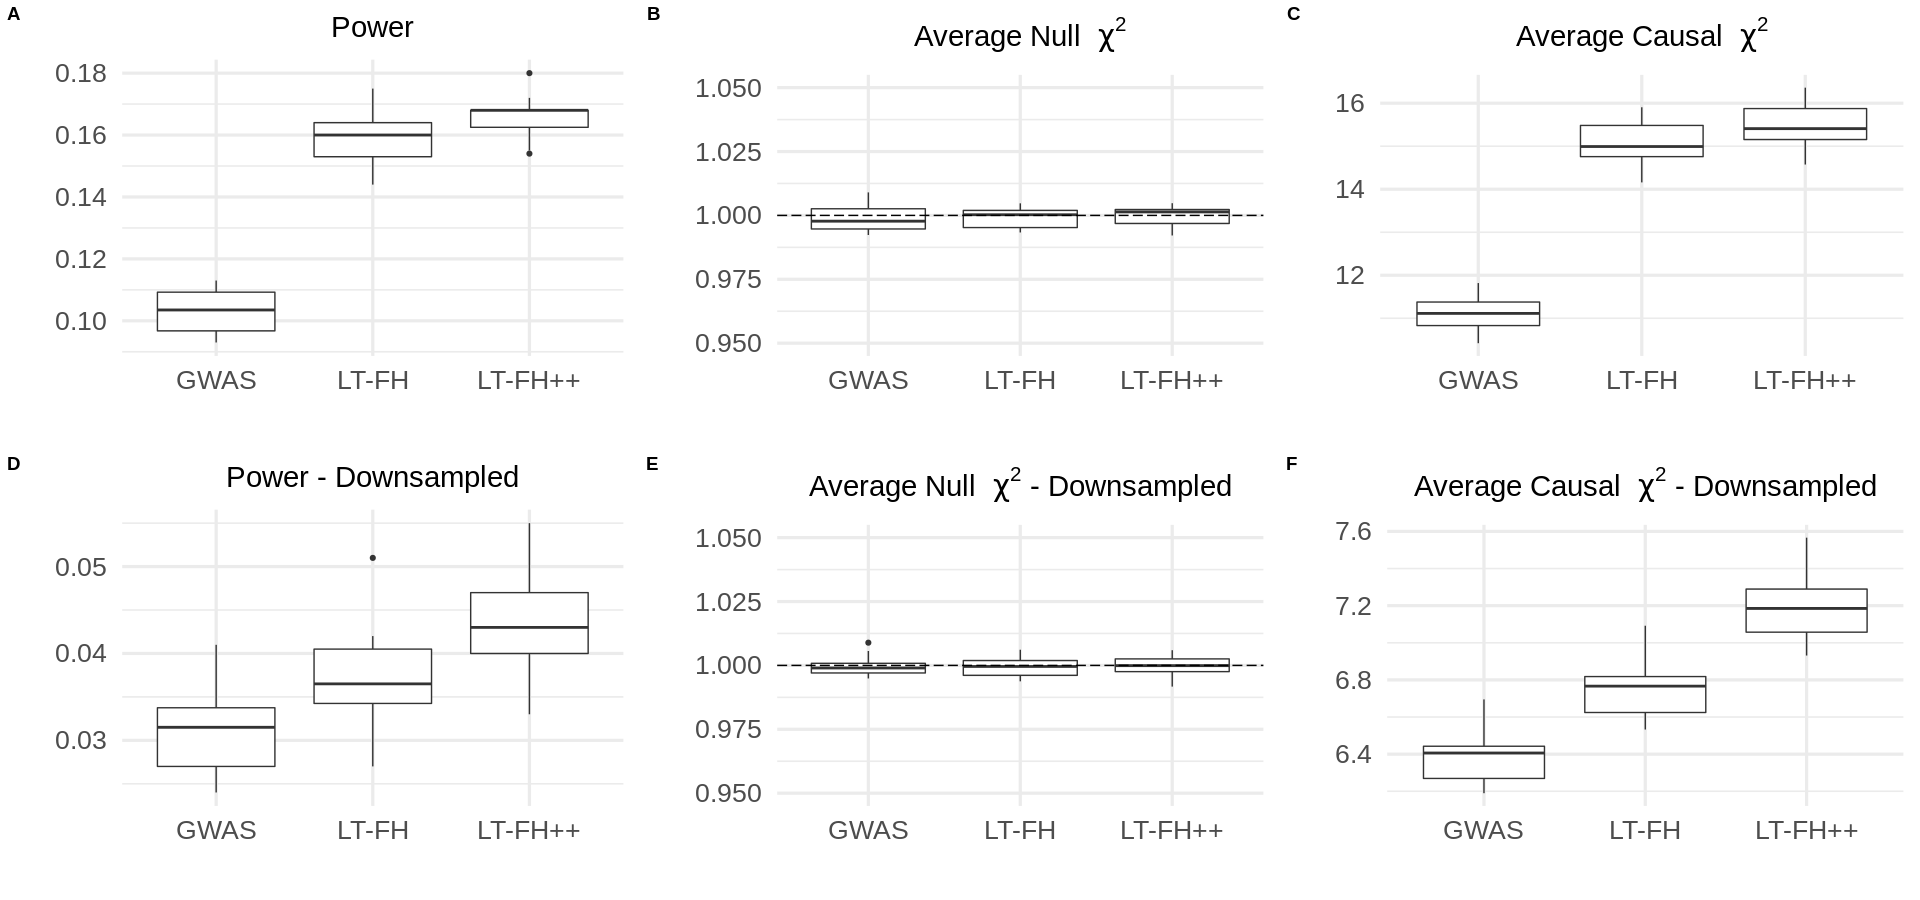
\includegraphics[width=\textwidth]{results/boxplot_05prev_both.png}
	\caption[Simulation results for a $ 5\% $ prevalence, with and without downsampling of controls]{Linear regression was used to perform the GWAS for LT-FH and LT-FH++, while a 1-df chi-squared test was used for case-control status. We assessed the power of each method by considering the fraction of causal SNPs with a p-value below $ 5 \times 10^{-8} $. Here, GWAS refers to case-control status and LT-FH and LT-FH++ are both without siblings. Downsampling refers to downsampling the controls such that we have the same number of cases and controls, i.e.\, we have $ 10,000 $ individuals in total for a $ 5\% $ prevalence and $ 20,000 $ individuals for a $ 10\% $ prevalence.}
	\label{fig:LTFHppSimulationResults}
\end{figure}

The simulations show a modest increase in favour of LT-FH++ over LT-FH in the full sample, with an average power increase across the $ 10 $ simulations of $ 4\% $. Both LT-FH and LT-FH++ has an average power increase of more than $ 50\% $ compared to the case-control status used in \textit{GWAS}, making either method vastly better. However, case ascertainment has a significant impact on the power ratio between LT-FH and LT-FH++. When case ascertainment is present in a biobank, the average power increase of LT-FH++ over LT-FH increased to $ 18\% $.

\newpage

\subsection{Real-world analysis}
\begin{wrapfigure}{O}{10cm}
	%	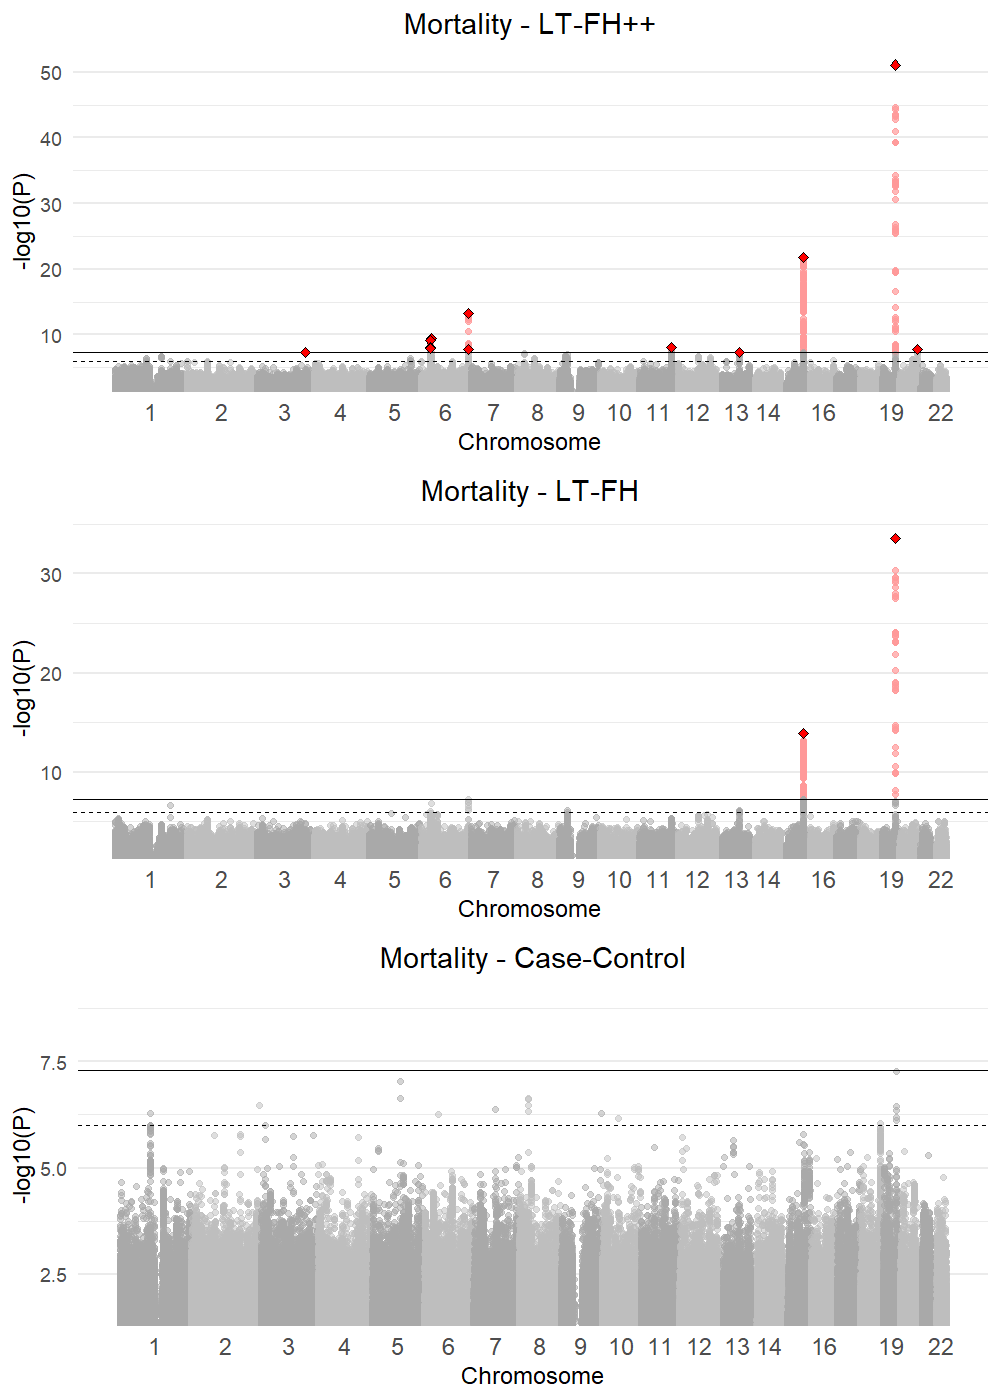
\includegraphics[width=0.7\textwidth]{results/manhattanPlot_mortality.pdf} % adds a lot of loading 
	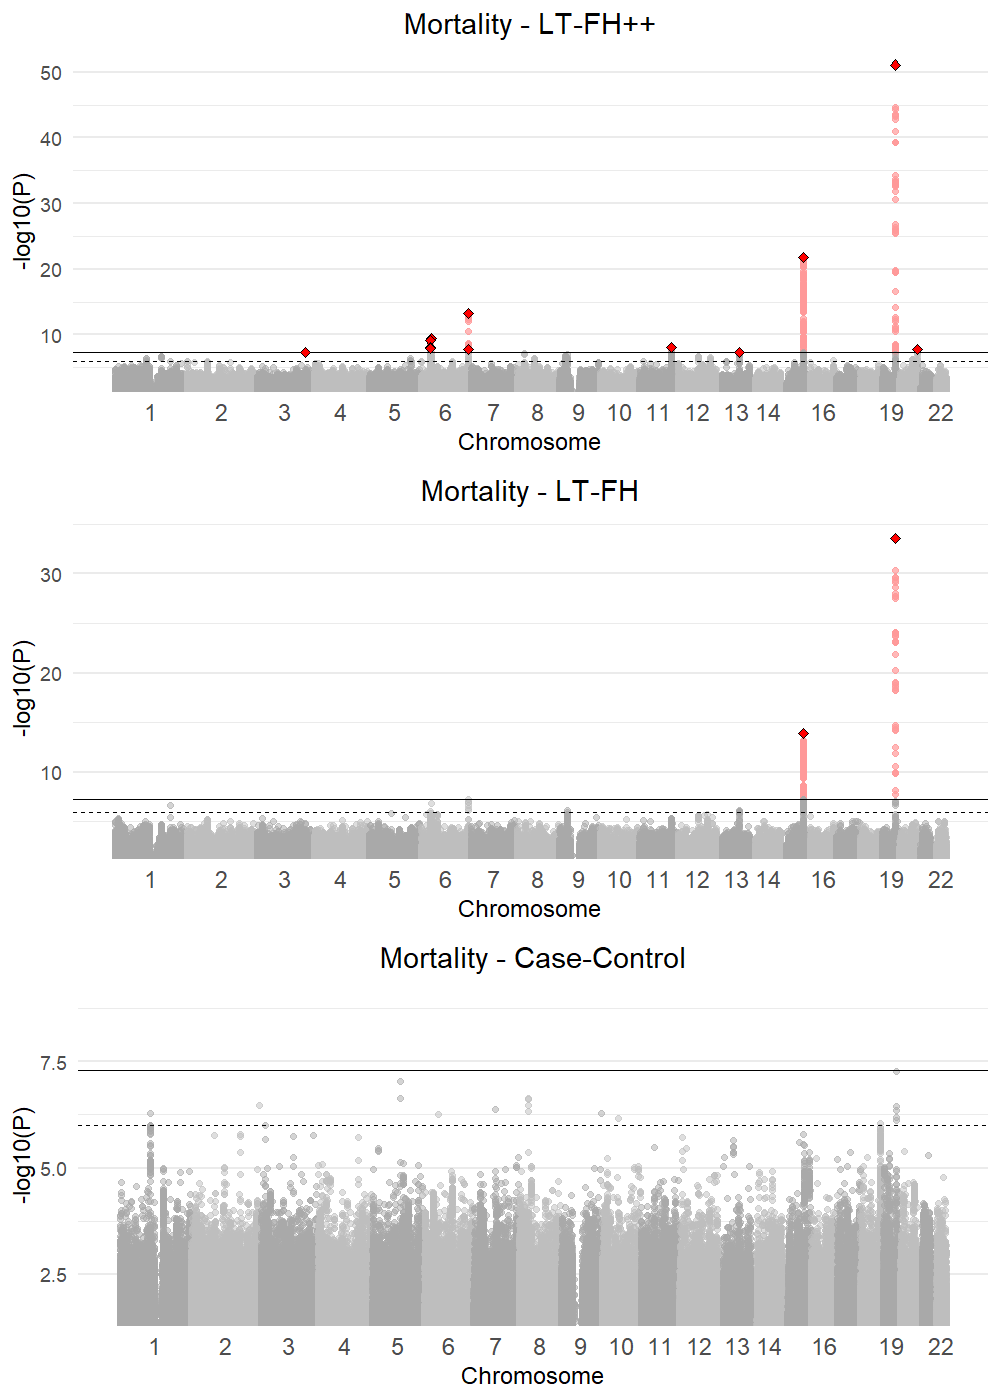
\includegraphics[width=10cm]{results/manhattanPlot_mortality.png}
	\caption[Manhattan plots for LT-FH++, LT-FH, and case-control GWAS of mortality	in the UK Biobank]{The Manhattan plots display a Bonferroni corrected significance level of $ 5\times 10^{-8} $ and a suggestive threshold of $ 5\times 10^{-6} $. The genome-wide significant SNPs are coloured in red. The diamonds correspond to top	SNPs in a window of size $ 300,000 $ base pairs.}
	\label{fig:LTFH++_manhattanMortality}
\end{wrapfigure}

LT-FH++ was also applied to four of the main psychiatric disorders in iPSYCH and to mortality in UKBB. The mortality GWAS in UKBB resulted in $ 0 $ genome-wide significant SNP for simple linear regression, $ 2 $ for LT-FH, and $ 10 $ for LT-FH++. The Manhattan plot for mortality can be found in \cref{fig:LTFH++_manhattanMortality}.

The GWAS in iPSYCH did not provide nearly as large of an increase in power for LT-FH++ or LT-FH over simple linear regression. In fact, we did not see any notable improvement over simple linear regression of the case-control status. The Manhattan plot for ADHD in iPSYCH can be found in \cref{fig:LTFH++_manhattanADHD}. We did find $ 7 $ genome-wide significant SNPs for ADHD using LT-FH++ and $ 5 $ for LT-FH and case-control status, but the two additional associations for LT-FH++ were very close to genome-wide significance for the other two outcomes as well.
\begin{wrapfigure}{R}{10cm}
	%	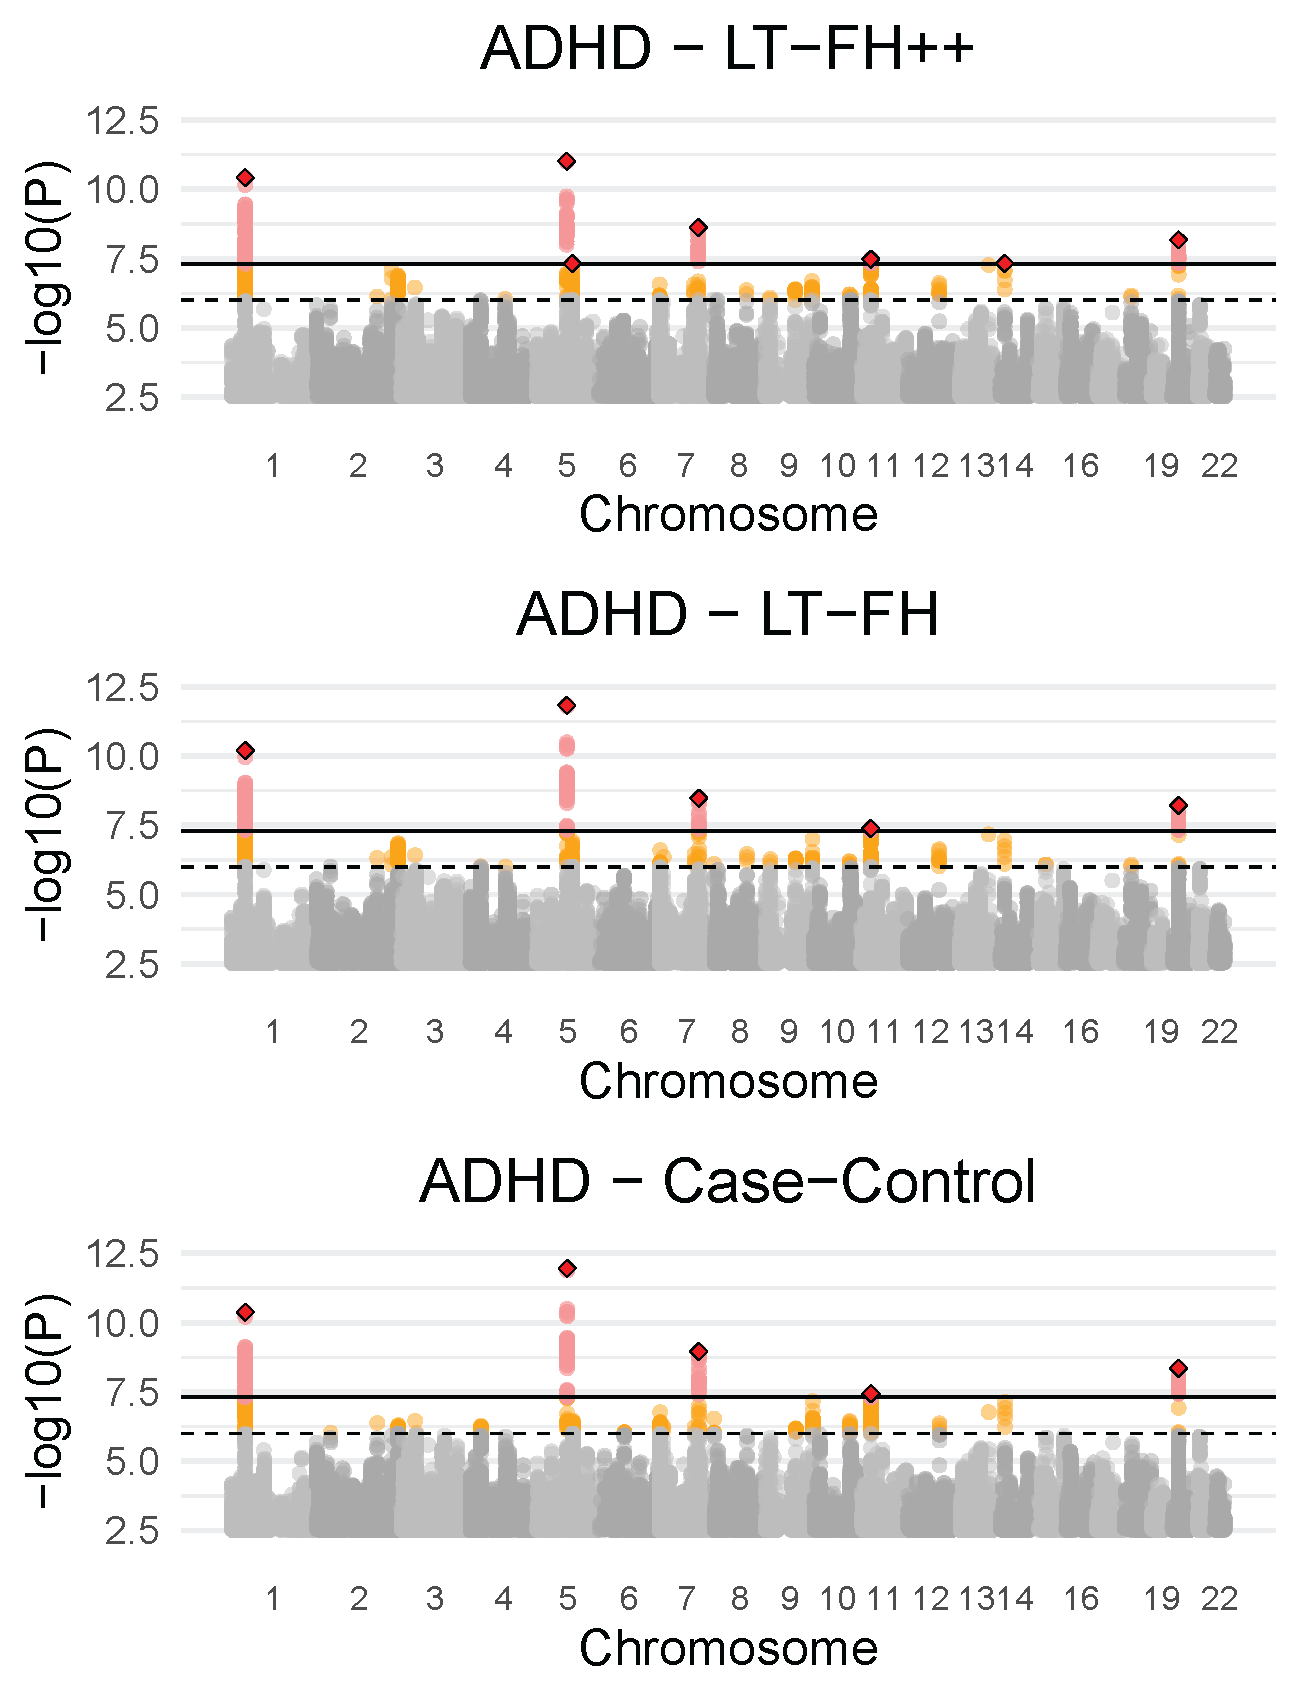
\includegraphics[width=0.7\textwidth]{results/manhattanPlot_ADHD.pdf} % adds a lot of loading 
	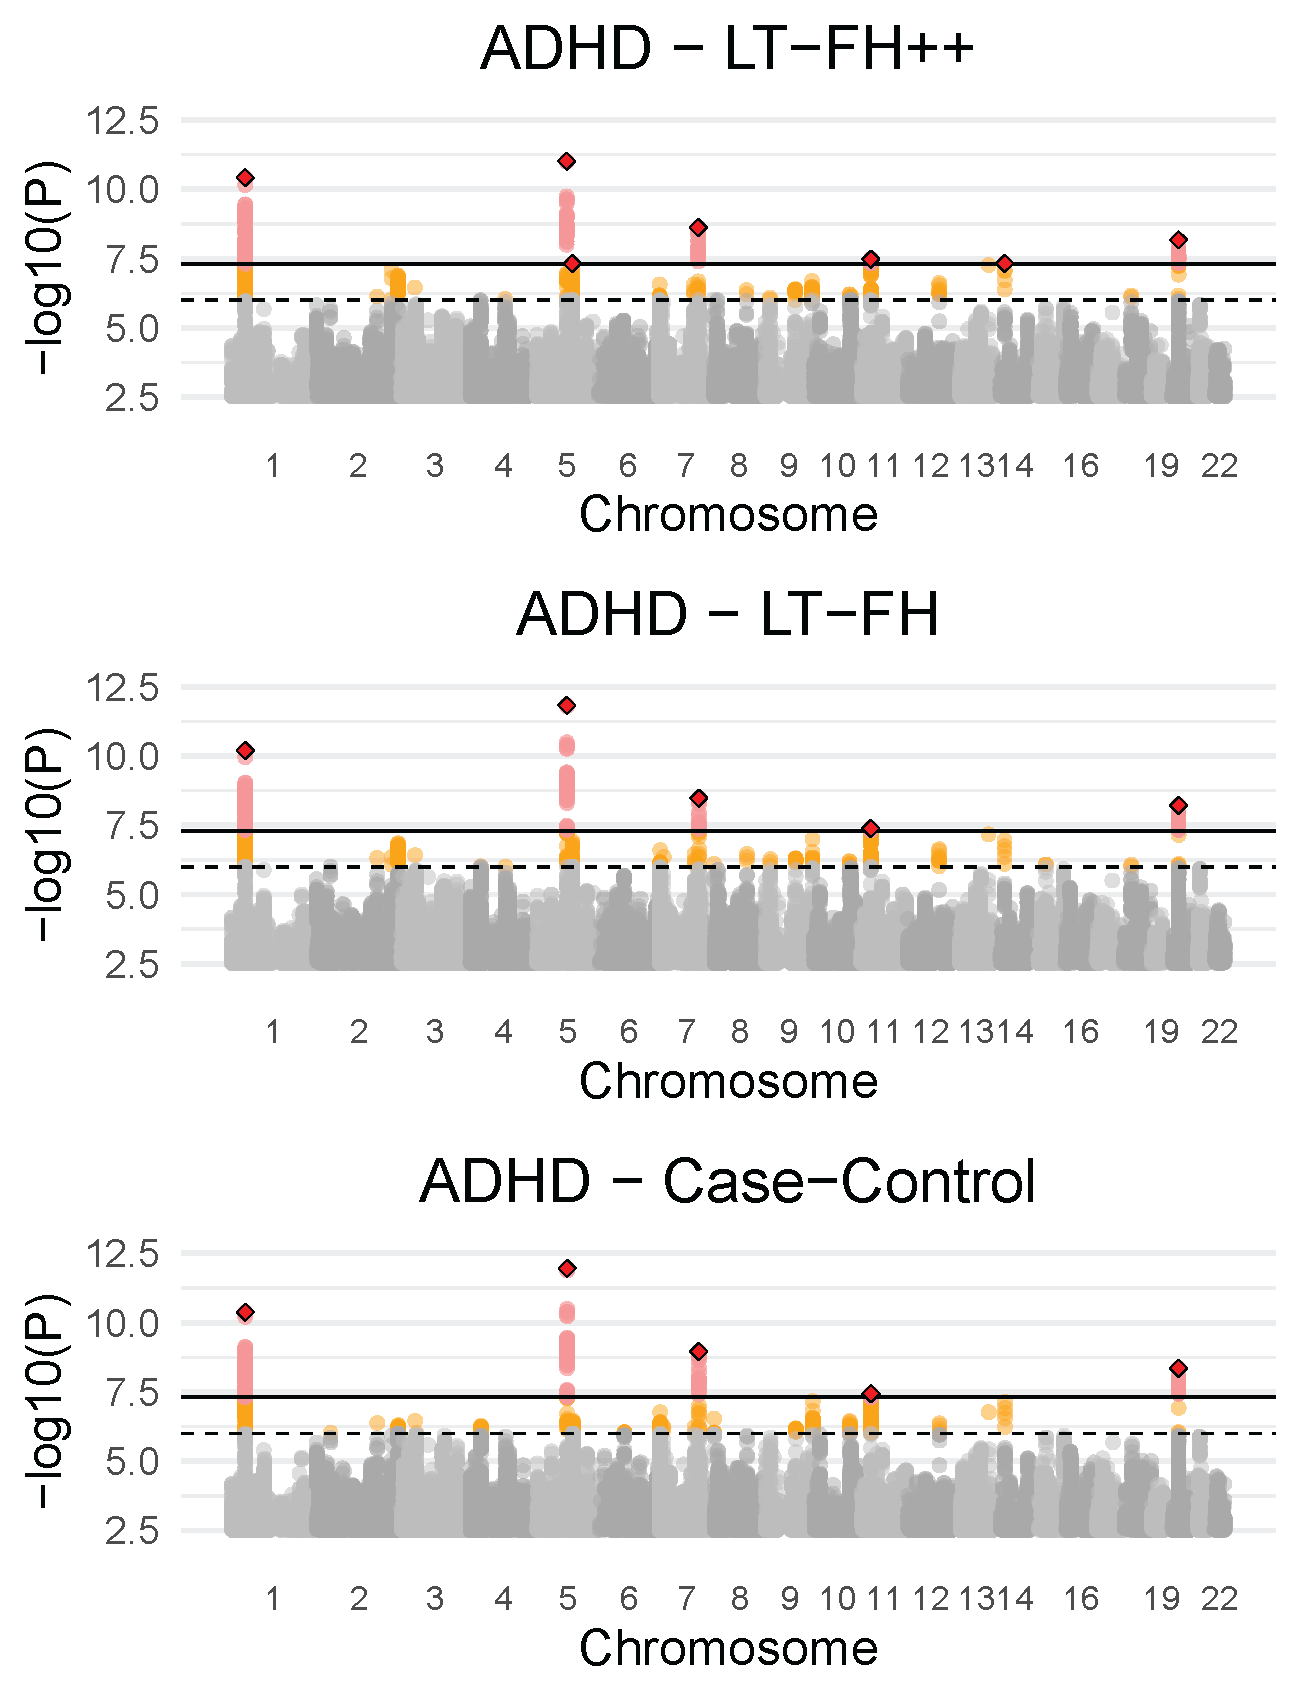
\includegraphics[width=10cm]{results/manhattanPlot_ADHD.png}
	\caption[Manhattan plots for LT-FH++, LT-FH, and case-control GWAS of ADHD in the iPSYCH data]{The dashed line indicates a suggestive p value of $ 5\times 10^{-6} $ and the fully drawn line at $ 5\times 10^{-8} $ indicates genome-wide significance threshold. The genome-wide significant SNPs are coloured in red. The diamonds correspond to top SNPs in a window of size $ 300,000 $ base pairs.}	
	\label{fig:LTFH++_manhattanADHD}
\end{wrapfigure}
Through additional simulations we found that one can expect the most \textit{relative} power gain with LT-FH++ over LT-FH if the in-sample prevalence is high in either family members or the index persons. This is because LT-FH++ is best able to utilise information for cases, since the CIPs provide a very accurate estimate for the full liability of an individual.
\newpage

\section{Paper 2 - ADuLT}
The second paper utilised the age-dependent liability threshold (ADuLT) model, which is the model underlying LT-FH++. The name change is in large part due to the focus on only the age-dependency and not family history, even though it is the same model. The purpose of the project was to examine the performance of the ADuLT outcome with established time-to-event GWAS methods that are based on the Cox proportional hazards (PH) model. It is two fundamentally different ways to approach time-to-event analysis in a GWAS setting. The adoption of Cox PH models in a GWAS setting has been limited, which has also been evident in the relative lack of method developments for Cox PH models compared to other regression models. Since one of the main limitations for Cox PH is the computational cost of such a model, GWAS with these models have been limited to less than $ 100,000 $ individuals. Recently, a method called SPACox \cite{bi2020fast} has been proposed that allows for far better scaling, and allowing for analysis of large biobanks. We will use SPACox as a representative of Cox PH models to compare to in this paper.

\subsection{Simulation results}

As for the first paper, we assessed the models in simulations first. We simulated the genotypes and assigned phenotypes with two generative models. The first model was the liability threshold model and the second model was the proportional hazards model. Notably, one would expect a method based on the liability threshold model to perform the best under this model, and subpar under other generative models. The simulation results shown in \cref{fig:adult_simulations} show the power for $ 10 $ replications under two different generative models and for different population prevalences. In \cref{fig:adult_simulations}A, the ADuLT or case-control status methods perform slightly better than the Cox PH model under the liability threshold model and vice versa, which is what we expected. Notably, there is no case ascertainment in those simulations. The results shown in \cref{fig:adult_simulations}B are with case ascertainment and we observe a large shift in power between methods under both generative models. In short, the simulation results show that the Cox PH based method has a far lower power than the LTM based methods under \textit{both} generative models, when cases are ascertained. Even after performing inverse probability weighing Cox PH on a select subset of null SNPs and all causal SNPs, we observed the same result. This indicates that the Cox PH models with the current implementation suffers from a significant power loss when case ascertainment is present in a GWAS setting, which is very common in practice.

%\begin{wrapfigure}{O}{10cm}
\begin{figure}[h]
	\centering
	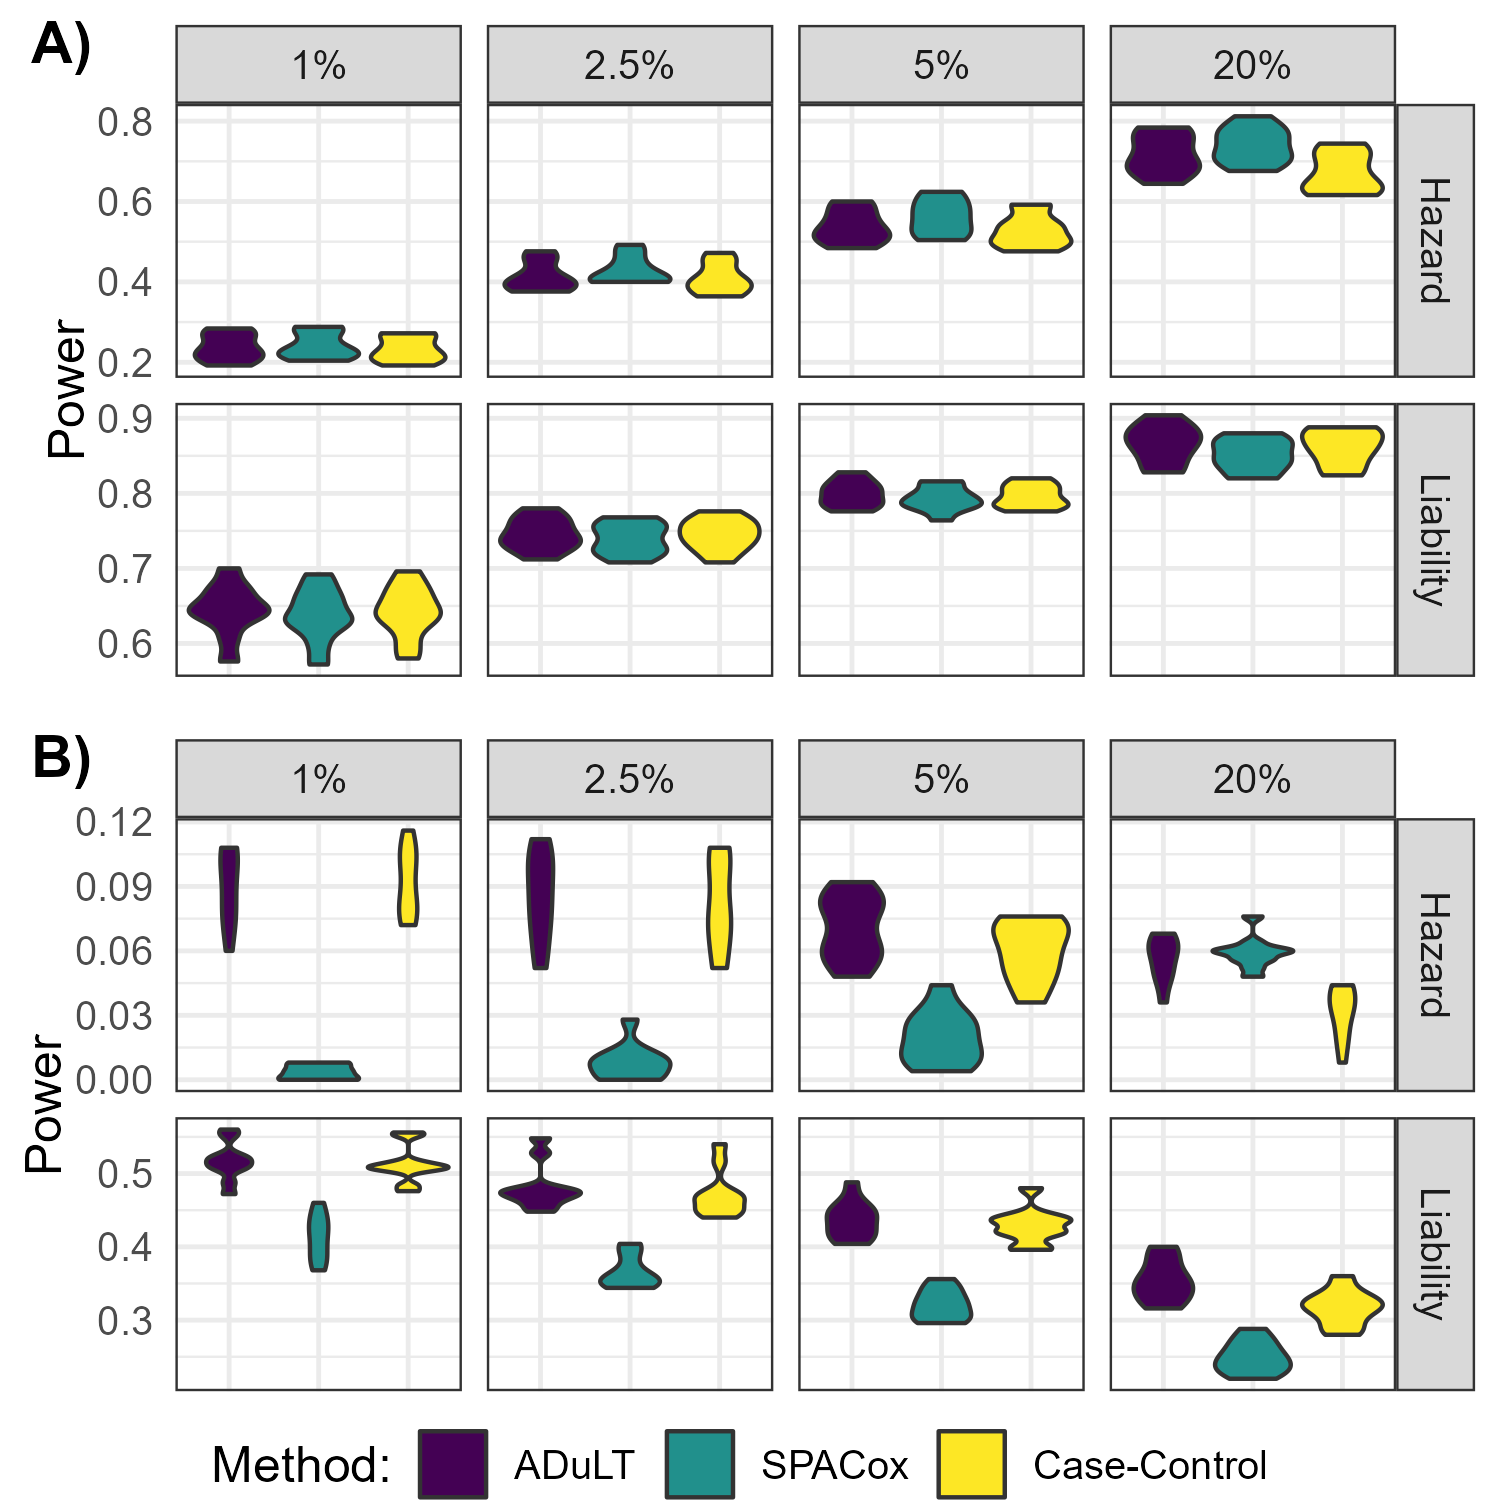
\includegraphics[width=10cm]{results/adult_combined_C250_power}
	\caption[Power simulation results with $ 250 $ causal SNPs under both generative models and varying prevalences.]{The power is shown for different population prevalence, varying from $ 1\% $ to $ 20\% $. \textbf{A)} The power, i.e.\ the fraction of causal SNPs detected for each method, \textbf{without downsampling}. \textbf{B)} The power \textbf{with downsampling}, i.e.\ the number of individuals is subsampled to 10k cases and 10k controls.}
	\label{fig:adult_simulations}
%\end{wrapfigure}
\end{figure}


\subsection{Real-world analysis}
Next, we applied the same analysis to real-world data to assess whether we observed the same behaviour with case ascertainment present in the data. iPSYCH is particularly useful for this, as all cases in a given time period have been sampled and sequenced, meaning the iPSYCH data has a high case ascertainment.

We found that the Cox PH model had a rather large loss of power compared to ADuLT and case-control status. Across the four analysed psychiatric disorders, ADuLT found $ 20 $ independent associations, case-control status found $ 17 $, and SPACox found $ 8 $. The ADHD Manhattan plots for the three methods compared in paper 2 can be found in \cref{fig:adult_ADHD}. In no circumstances did the Cox PH model outperform a LTM based method, showing that the currently implementation of Cox PH model does not perform as well as simpler models such as linear regression, which are also far more computationally efficient.

%\begin{wrapfigure}{O}{10cm}
\begin{figure}[h] 
	\centering
	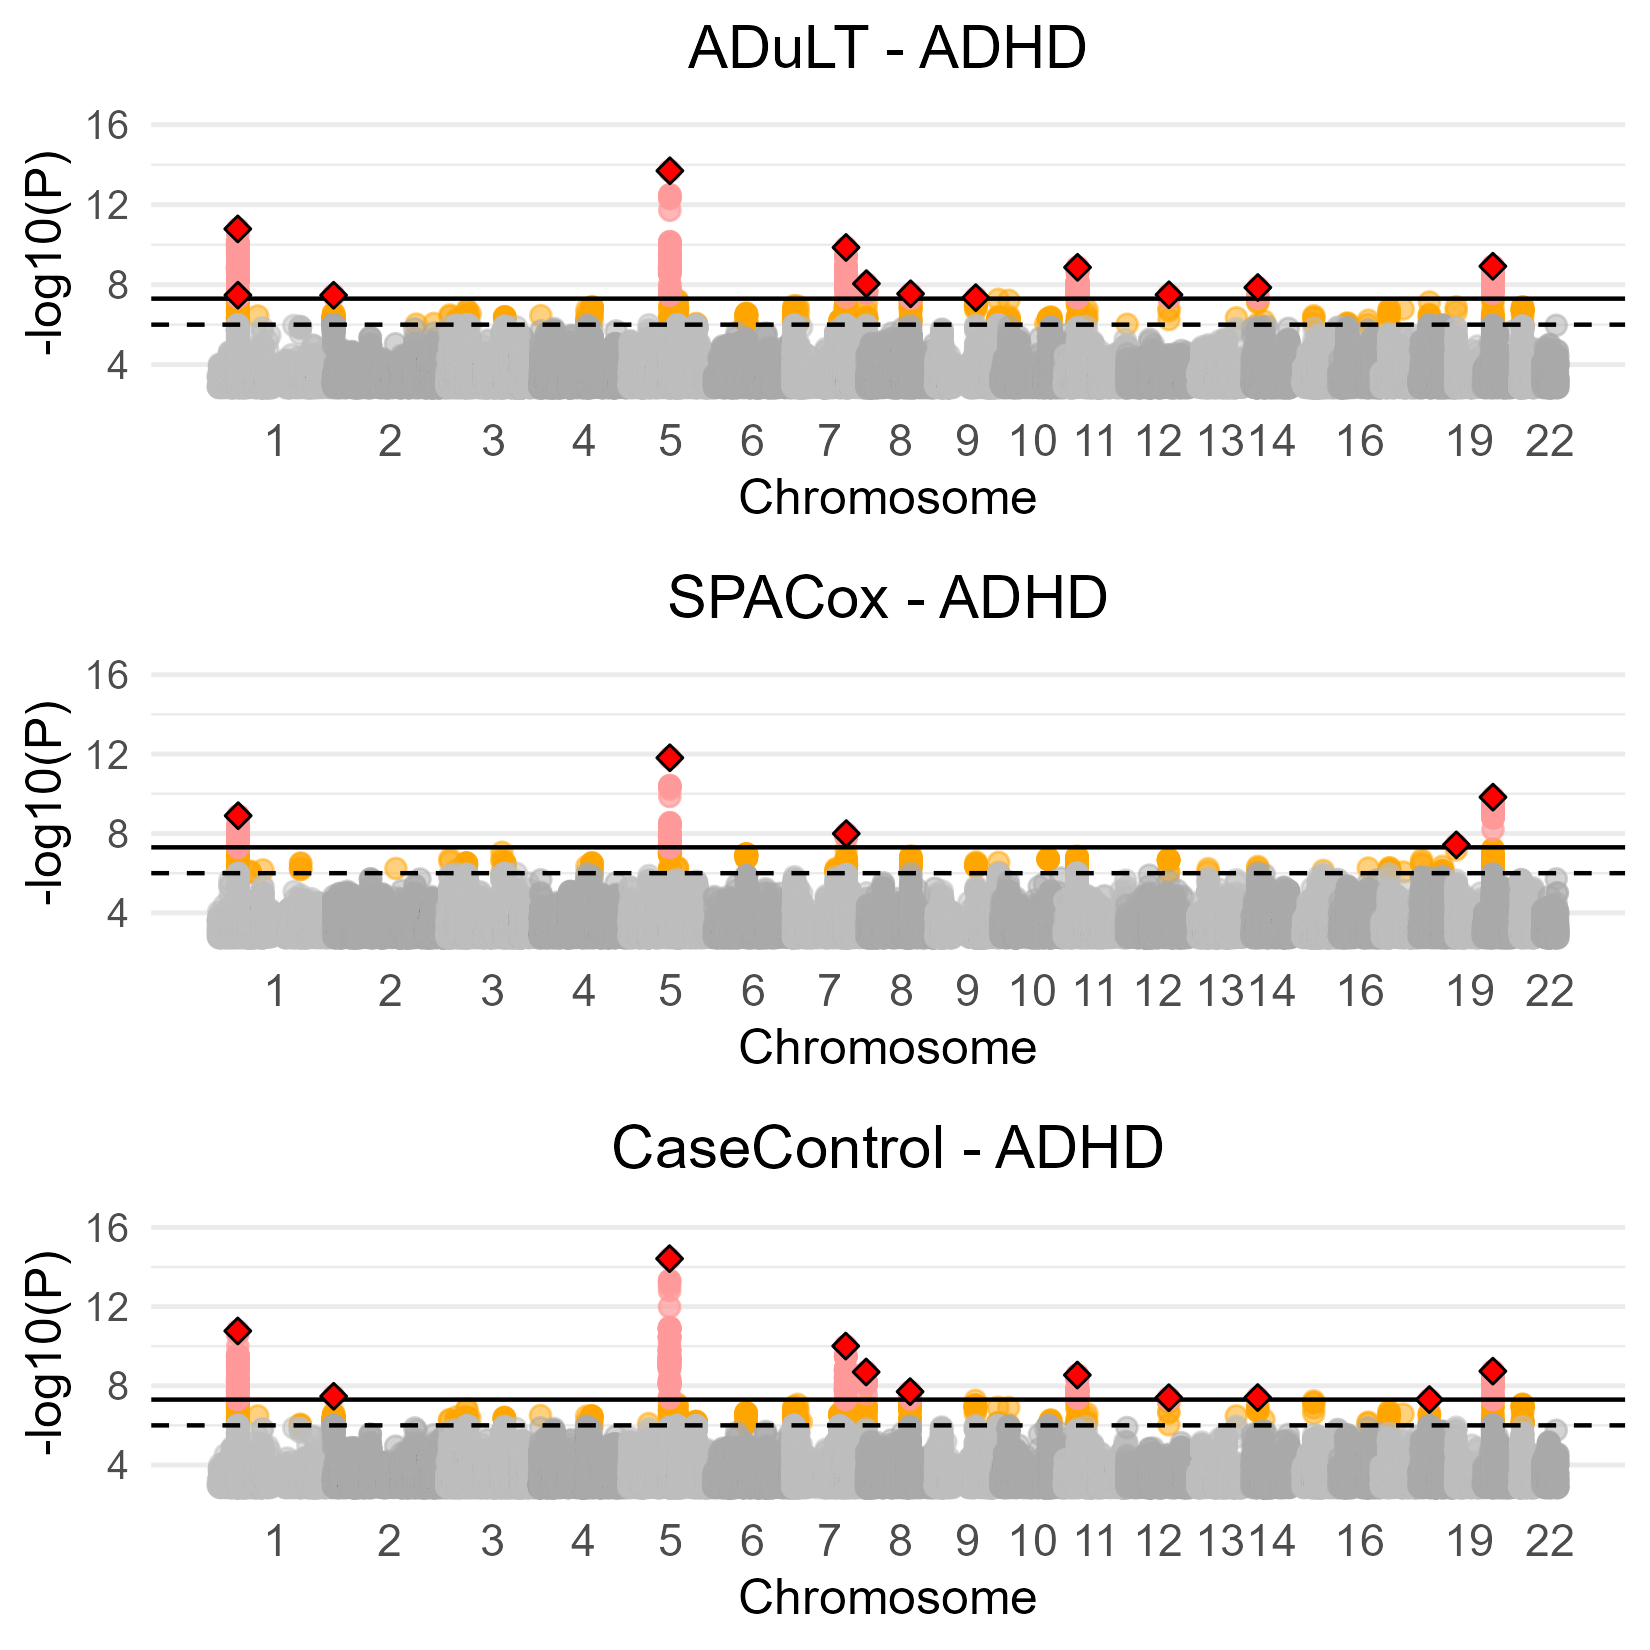
\includegraphics[width=10cm]{results/adult_manhattanPlot_ADHD}
	\caption[Manhattan plots from GWAS with the ADuLT phenotype, SPACox, and case-control status for ADHD]{Manhattan plots for ADHD for all three methods. Case-control GWAS uses the age of individuals as a covariate, whereas the ADuLT GWAS and SPACox do not. The orange dots indicate suggestive SNPs with a p-value threshold of $ 5 \times 10^{-6} $. The red dots correspond to genome-wide significant SNPs with a p-value threshold of $ 5 \times 10^{-8} $. The diamonds correspond to the lowest p-value LD clumped SNP in a 500k base pair window with an $ r^2 = 0.1 $ threshold.}
	\label{fig:adult_ADHD}
%\end{wrapfigure}
\end{figure}


\newpage

\section{Paper 3 - fGRS}
The final paper does not focus on GWAS, but rather on the predictive value of the LT-FH++ phenotype as an alternative to the conventional binary family history variable in prediction models. In epidemiology, family history is a well-known and powerful predictor that has been used to improve prediction models of complex phenotypes such as mental disorders, suicide, and heart disease. As the intension is to provide an estimate of an individual's liability for a given disorder before getting an actual diagnosis, we will not consider the case-control status of the index person, but only the family members. In many ways this is similar to the purpose of the PRS and how it is currently being used to screen individuals for disorders. However, instead of using the individual's genotypes to acquire an aggregate genetic risk score, we will use the family history to estimate a liability. 

\subsection{Real-World Analysis}

\begin{wrapfigure}{O}{10cm}
	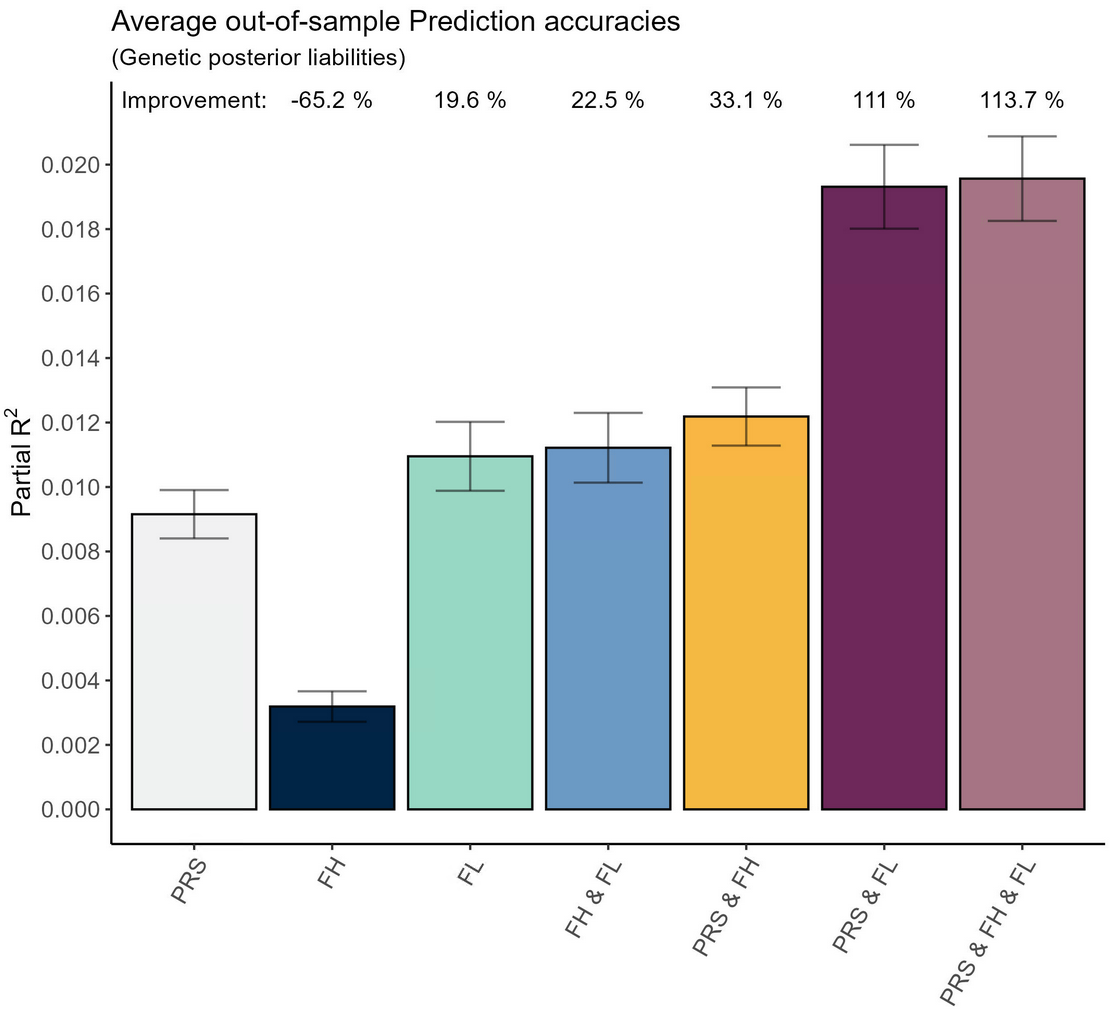
\includegraphics[width=10cm]{results/avg_partial_prediciton_accuracies_noED.png}
	\caption[Average out of sample prediction across $ 8 $ disorders]{
		\sl Average partial $ R^2 $ across $ 8 $ disorders with various prediction models. We excluded eating disorders from the average, as hardly any family history was present for these disorders. The base model includes age, sex, and $ 20 $ PCs. \textit{PRS} refers to the base model with the PRS included as well. \textit{FH} refers to the base model with the binary family history, and \textit{FL} refers to the LT-FH++ variable. Combinations of these variables are presented as \textit{PRS} \& \textit{FH} for the model with PRS and the binary family history variable etc..}
	\label{fig:paper3:predictionResults}
\end{wrapfigure}

We will consider a base model that contains the index person's sex, age, and $ 20 $ PCs. We will add additional predictors to the base model and assess the additional predictive value of each predictor. We will use the partial $ R^2 $ as a measure of predictive value. From the additional predictors and combinations of them, we can derive the best family history variable and the best overall model. We will consider the PRS for a given disorder, as well as a binary family history indicator or the LT-FH++ phenotype (but with the index person's status removed). We present the results in \cref{fig:paper3:predictionResults}. We calculated the average partial $ R^2 $ across $ 8 $ phenotypes available to iPSYCH, but we left out eating disorders, as there were almost no family history available. We find that the LT-FH++ phenotype provided a $ 19.6\% $ increase over the the PRS model, while the binary family history variable had a predictive value $ 65.2\% $ lower than the PRS model. Of the models with only two predictors, the best model was the one with the PRS and LT-FH++ phenotype predictors. They had an average partial $ R^2 $ of $ 111\% $ across the $ 8 $ disorders, resulting in a partial $ R^2 $ value that is close the sum of each predictor. The model with both family history variables had almost the same predictive value as the model with only the LT-FH++ variable, indicating that most of the predictive value is captured by the LT-FH++ phenotype. The same is also true for the model where both family history variables and the PRS is included. It is very close to the predictive value of the model with only the LT-FH++ phenotype and the PRS.

\subsubsection{Multi-Trait Prediction}

\begin{wrapfigure}{O}{10cm}
	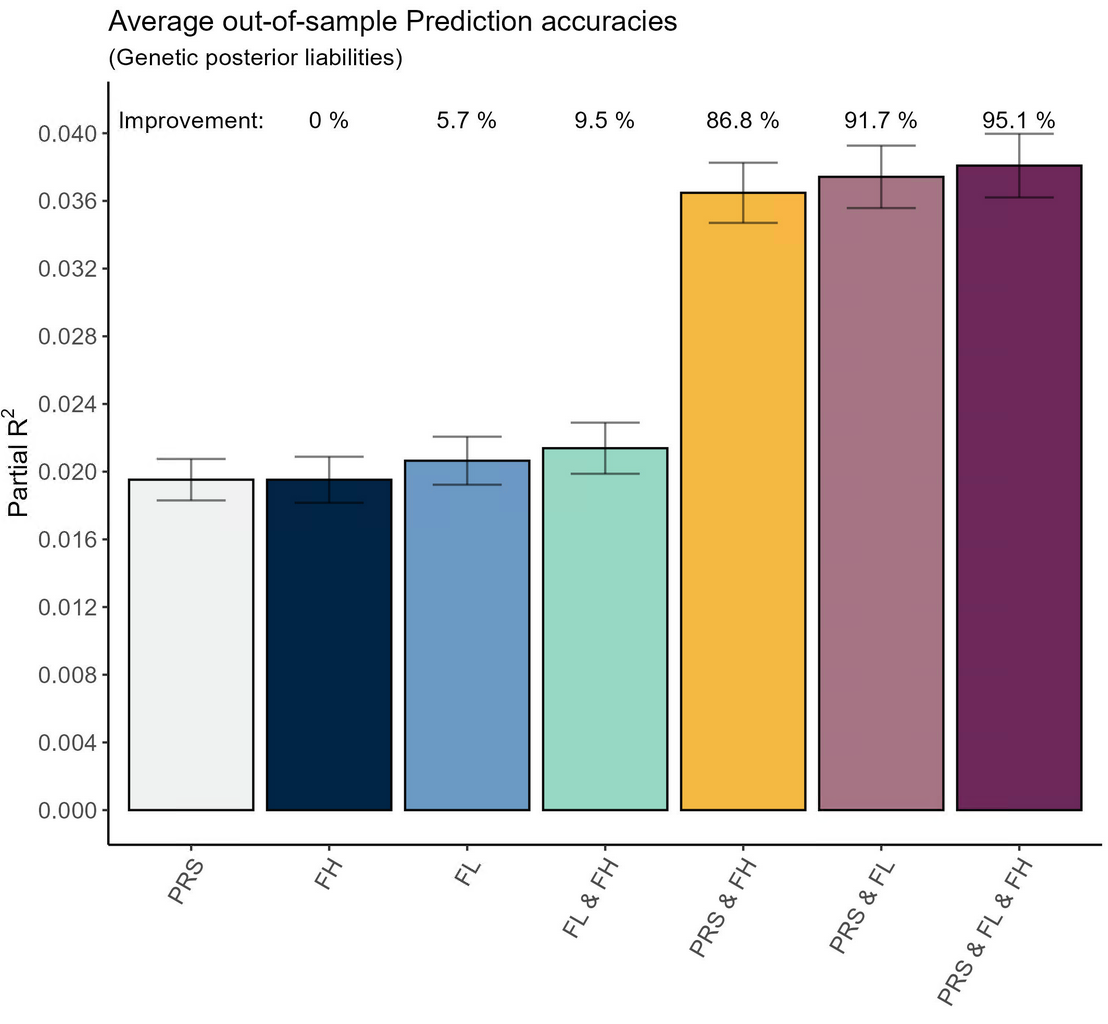
\includegraphics[width=10cm]{results/avg_partial_prediciton_accuracies_multi_trait.png}
	\caption[Average out of sample prediction for multi trait]{
		\sl Average partial $ R^2 $ across $ 5 $ disorders with various prediction models. The base model includes age, sex, and $ 20 $ PCs. As the prediction is based on multi trait, \textit{PRS} refers to the base model with the PRS of all considered phenotypes included. \textit{FH} refers to the base model with all binary family history variables included, and \textit{FL} refers to the model with all LT-FH++ variables included. Combinations of these variables are presented as \textit{PRS} \& \textit{FH} for the model with all PRSs and all binary family history variables etc..}
	\label{fig:paper3:predictionResultsMultiTrait}
\end{wrapfigure}

On top of this, we will also considered correlated phenotypes. Mental disorders are notoriously difficult to diagnose and many mental disorders have a high genetic correlation. Accounting for correlated phenotypes is therefore an attempt at utilising the information from the highly correlated phenotypes to improve prediction. For correlated trait, we restricted to the iPSYCH disorders. This was done due to the requirement of genetic correlations, which has already been calculated by Schork et al.\cite{schork2019genome}. In order to have as fair of a comparison as possible, we also created multi trait models for the other predictors. For instance, we considered a multi trait PRS model, which is a model with the PRS of all the considered correlated phenotypes. Similarly, the binary family history variable for all the correlated phenotypes was also included. For LT-FH++, we considered two scenarios. The first is the correlated phenotype extension as presented in \cref{sec:methods:ltfhpp:correlatedTraits}. It resulted in a single liability estimate that represents the family history for all of the considered disorders. We also considered a simpler approach, where the single trait LT-FH++ phenotype was included for each of the considered phenotypes. The first approach for LT-FH++ did not perform as well as the other methods, and will not be presented here. Therefore, we used the single trait LT-FH++ phenotype for each of the considered phenotypes. The multi trait results are presented in \cref{fig:paper3:predictionResultsMultiTrait}. 



When considering multiple traits, we did not observe any difference in predictive value between the considered PRSs and binary family history variables. The model with multiple single trait LT-FH++ phenotypes had a slightly higher predictive value, which was $ 5.7\% $ higher than the other two. As with the single trait prediction models, the model with both family history variables did not increase the predictive value, meaning most of the predictive value is captured by either of the family history variables. However, when considering a model with the multi trait PRS variables and either of the multi trait family history variables, we observe close to a doubling of the predictive value. This indicates that most of the predictive value caught by the PRS and family history models is different. The model with all three predictors has almost the same predictive value of the model with the PRS and either of the family history variables.



\newpage



%\begin{enumerate}
%%	\item LT-FH++: highlight Mortality and ADHD. It shows the importance of including family history and age-of-onset to increase 
%%power, but also shows that it is not the end all be all.
%%	\begin{enumerate}
%%		\item Mortality GWAS - large power increase
%%		\item ADHD GWAS - almost no power increase
%%	\end{enumerate}
%%	\item ADuLT: when only looking at age-of-onset, cox PH models are probably not the best model to use. ADuLT is \textit{never} the 
%%worst model, but also not always the best. The most robust method is ADuLT, since power is always best or close to the best.
%%	\begin{enumerate}
%%		\item simulation results with downsampling
%%		\item ADHD GWAS results
%%	\end{enumerate}
%%	\item fGRS: the predictive performance of the liabilities compared to binary variables.
%%	\begin{enumerate}
%%		\item single trait performance
%%		\item multi trait performance 
%%		\item cross ancestry performance
%%	\end{enumerate}	
%	\item Do I need a section combining the results into a larger picture somehow here ? or is it meant to go in the discussion?
%\end{enumerate}
